\documentclass[thesis.tex]{subfiles}
\begin{document}
\chapter{Background}

\section{The mobile ecosystem}\label{sec:mobile-ecosystem}

This dissertation talks about the policies surrounding \emph{mobile
ecosystems}; but what, precisely, do we mean by the \emph{mobile
ecosystem}?  Succinctly when we refer to the mobile ecosystem we are
referring to \textbf{the interactions surrounding the use of smart
phones and tablet computers}.  Figure~\ref{fig:mobile-ecosystem} shows
some of the relationships between devices, their users and their
preferences, the stores, companies and all these principal's
policies. Users have phones or other mobile devices.  They may own
personal devices or have a company one.  They may have their own
preferred ways of using the device, or they may be subject to policies
written for their employer.  They download apps, written by developers
from app stores, all with their own policies and some of the stores
may delegate some aspects of their quality control to external vetting
software.  Even just describing these aspects of the mobile ecosystem
\autoref{fig:mobile-ecosystem} is quite complex.

To fully understand the scale of the mobile ecosystem, however, it is
best to describe some of the history surrounding it.

\begin{figure}
  \centering
  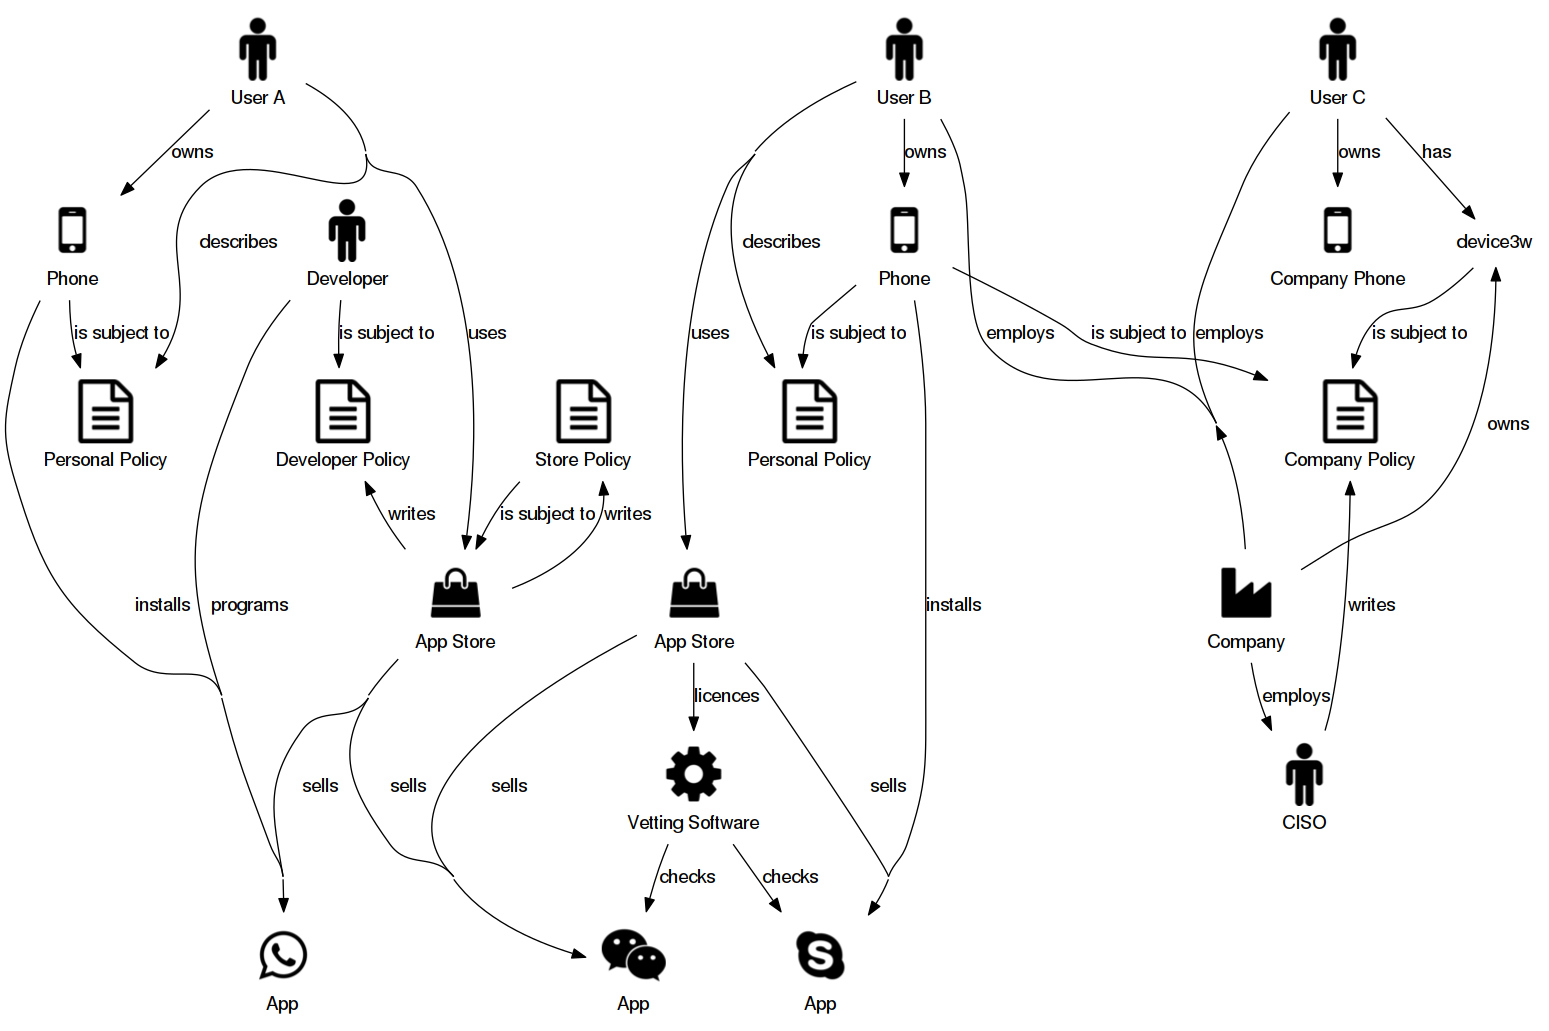
\includegraphics[width=\linewidth]{figures/mobile-ecosystem.png}
  \caption{Interactions between surrounding the use of mobile devices.}
  \label{fig:mobile-ecosystem}
\end{figure}

\subsection{Mobile devices: the story so far}

Some of the earliest mobile devices were the \acp{PDA} devices of the
early 90s.  The earliest devices, such as Apple's Newton, were
portable miniature computers designed to store personal information,
calendars and notes.  Developers could even program additional apps
for them (in the case of the Newton using Apple's Dylan language).  At
the time mobile phones were just portable telephones, but starting
with the IBM Simon in 1994 these devices started to have some of the
functionality of the \ac{PDA}, becoming what would later be called a
\emph{smart phone}.  The big advantage of these early smart phones
over the \ac{PDA} was they had a telephone connection.  The earliest
devices allowed their users to access email and fax, as well as
managing personal information.  The early smart phones were somewhat
underpowered compared to the \ac{PDA} devices so both continued to
develop alongside one another, and started to become more affordable.

In 1998 the Symbian OS was released.  Developed by Psion (who made
\acp{PDA}), and Motorola, Ericsson and Nokia (all phone
manufacturers).  By the early 2000s it would start to become the
dominant smart phone OS.  These devices could install apps, written in
C++ or Java (if the phone supported JME). They had cameras, could play
music. They even had early malware which would illicitly send texts to
premium rate numbers.  They were the forebears of the \emph{modern}
smart phone.
They were also starting to become affordable, with the lowest end
models starting to being affordable by children and
teenagers\footnote{If you saved up for what seemed like
  forever$\ldots$}.  Devices like Nokia's N-Gage were marketed directly
towards these younger users and featured games users could buy for
their devices.

In the mid-2000s we first start to see the mobile
ecosystem proper.  We have users with different devices, downloading
apps from different sources (some pirated).  These devices
contained personal information of the \acp{PDA}, but also photographs
and music.  Users could browse the web, and send each other pictures.
With increasing amounts of personal information malware authors
started to take note.  In a blog post from 2006 for Symantec, Chien
noted~\cite{eric_chien_spyware_2006}:

\begin{quote}
  ``While threats exist and are actively spreading, we are probably
  still years away from the situation we have with the Microsoft Windows
  [$\cdots$] We have already seen spyware applications for mobile devices
  (e.g. Spyware.Flexispy) that can monitor activities on the mobile
  device and then send them to a remote server. [$\cdots$] Just as
  worrying is the fact that the adware market is just beginning to take
  notice of mobile devices. Already some Bluetooth advertising schemes
  have been tested, where a bus stop is outfitted with a device that
  just spams out messages via Bluetooth.

  [$\cdots$]
  
  So, while worms and Trojans already exist for the mobile
  platforms, spyware and adware applications are just now gaining a
  foothold in the mobile device space. Spyware and adware pose a
  potentially large security issue in the near future, as the companies
  that produce such applications are less affected by the natural
  limiting factors.''
\end{quote}

In 2008 Apple released the first iPhone, and shortly after Google
released the Android OS.  Symbian would release its final version in
2012, with Android as the dominant OS on most devices.  These
operating systems differed from past efforts, and conventional desktop
OS, in that they were far more controlled than previous systems.
Apple's devices could not run code that Apple had not signed or
install software from outside of its App Store, which Apple
controlled.  Android devices offered a similar app marketplace, but
where there seemed to be less checking of individual
apps~\cite{oberheide_dissecting_2012}. Whilst Android users could
install software from other sources, the option was hidden by default.
As well as restrictions to software, these devices were also better
protected.  Devices no longer had an all powerful \emph{root} account.
APIs were provided that restricted malicious behaviors.  One example
was stopping SMSs being sent programatically to premium rate accounts;
essentially ending a monetization technique that had been prevelent in
malware before. 

Mobile devices stored a large amount of personal data about their
users.  They contained address books, records of phone calls, and GPS
logs of where their users had been.  With iOS and Android user's
became more aware about privacy on their devices, in part because of
increased media coverage of privacy issues.  A survey in 2012 by
Chin~et~al{.} found that users were more concerned about privacy on
their mobile devices, than on their
laptops~\cite{chin_measuring_2012}. Users of a smartphone were more
likely to install an app that came recommended from a friend, was
popular or was free.  To subsidize the cost of producing free apps,
and to better understand how users used their apps, some developers
added adware and tracking libraries to their apps.  These libraries
accomplished a variety of tasks ranging from crash and error tracking,
to collecting personal data to be sold to advertisers to subsidize the
app's price~\cite{seungyeop_han_study_2012}.

This dynamic between users who were increasingly concerned about their
privacy and apps which were increasingly privacy invading, lead many
to argue that the mobile device operating systems needed better
controls for what data and permissions an app could
have~\cite{leontiadis_dont_2012}.  Many different schemes were
suggested to fix this and provide finer privacy
controls~\cite{jeon_dr._2012,beresford_mockdroid:_2011,conti_crepe:_2010,backes_appguard_2013}
(some of which will be described further in
\autoref{chap:related-work}).  In general, however, users did not
really understand the how app permissions
worked~\cite{felt_android_2012}.  By 2017 (and the present day) iOS
and Android had settled on a model where user's were asked by their
devices if an app could access certain data when it first requested it
and then the user could revoke that decision later if they wished.
Despite the present Android permissions model being \emph{ask on use},
a large number of older Android devices are still being used.  In June
2016 only 10\% of devices used the latest version of Android, with
around 5\% using a version more than five years old
(\autoref{fig:android-versions}).  In contrast 79\% of iOS devices use
the latest OS, 16\% use the previous version and only 5\% use anything
older~\cite{apple_app_2017}.  The greater fragmentation of the Android
versions has been attributed to the greater number of Android device
manufacturers each with their own update mechanisms as compared to
with iOS where Apple exclusively control and update all devices.

\begin{figure}
\centering
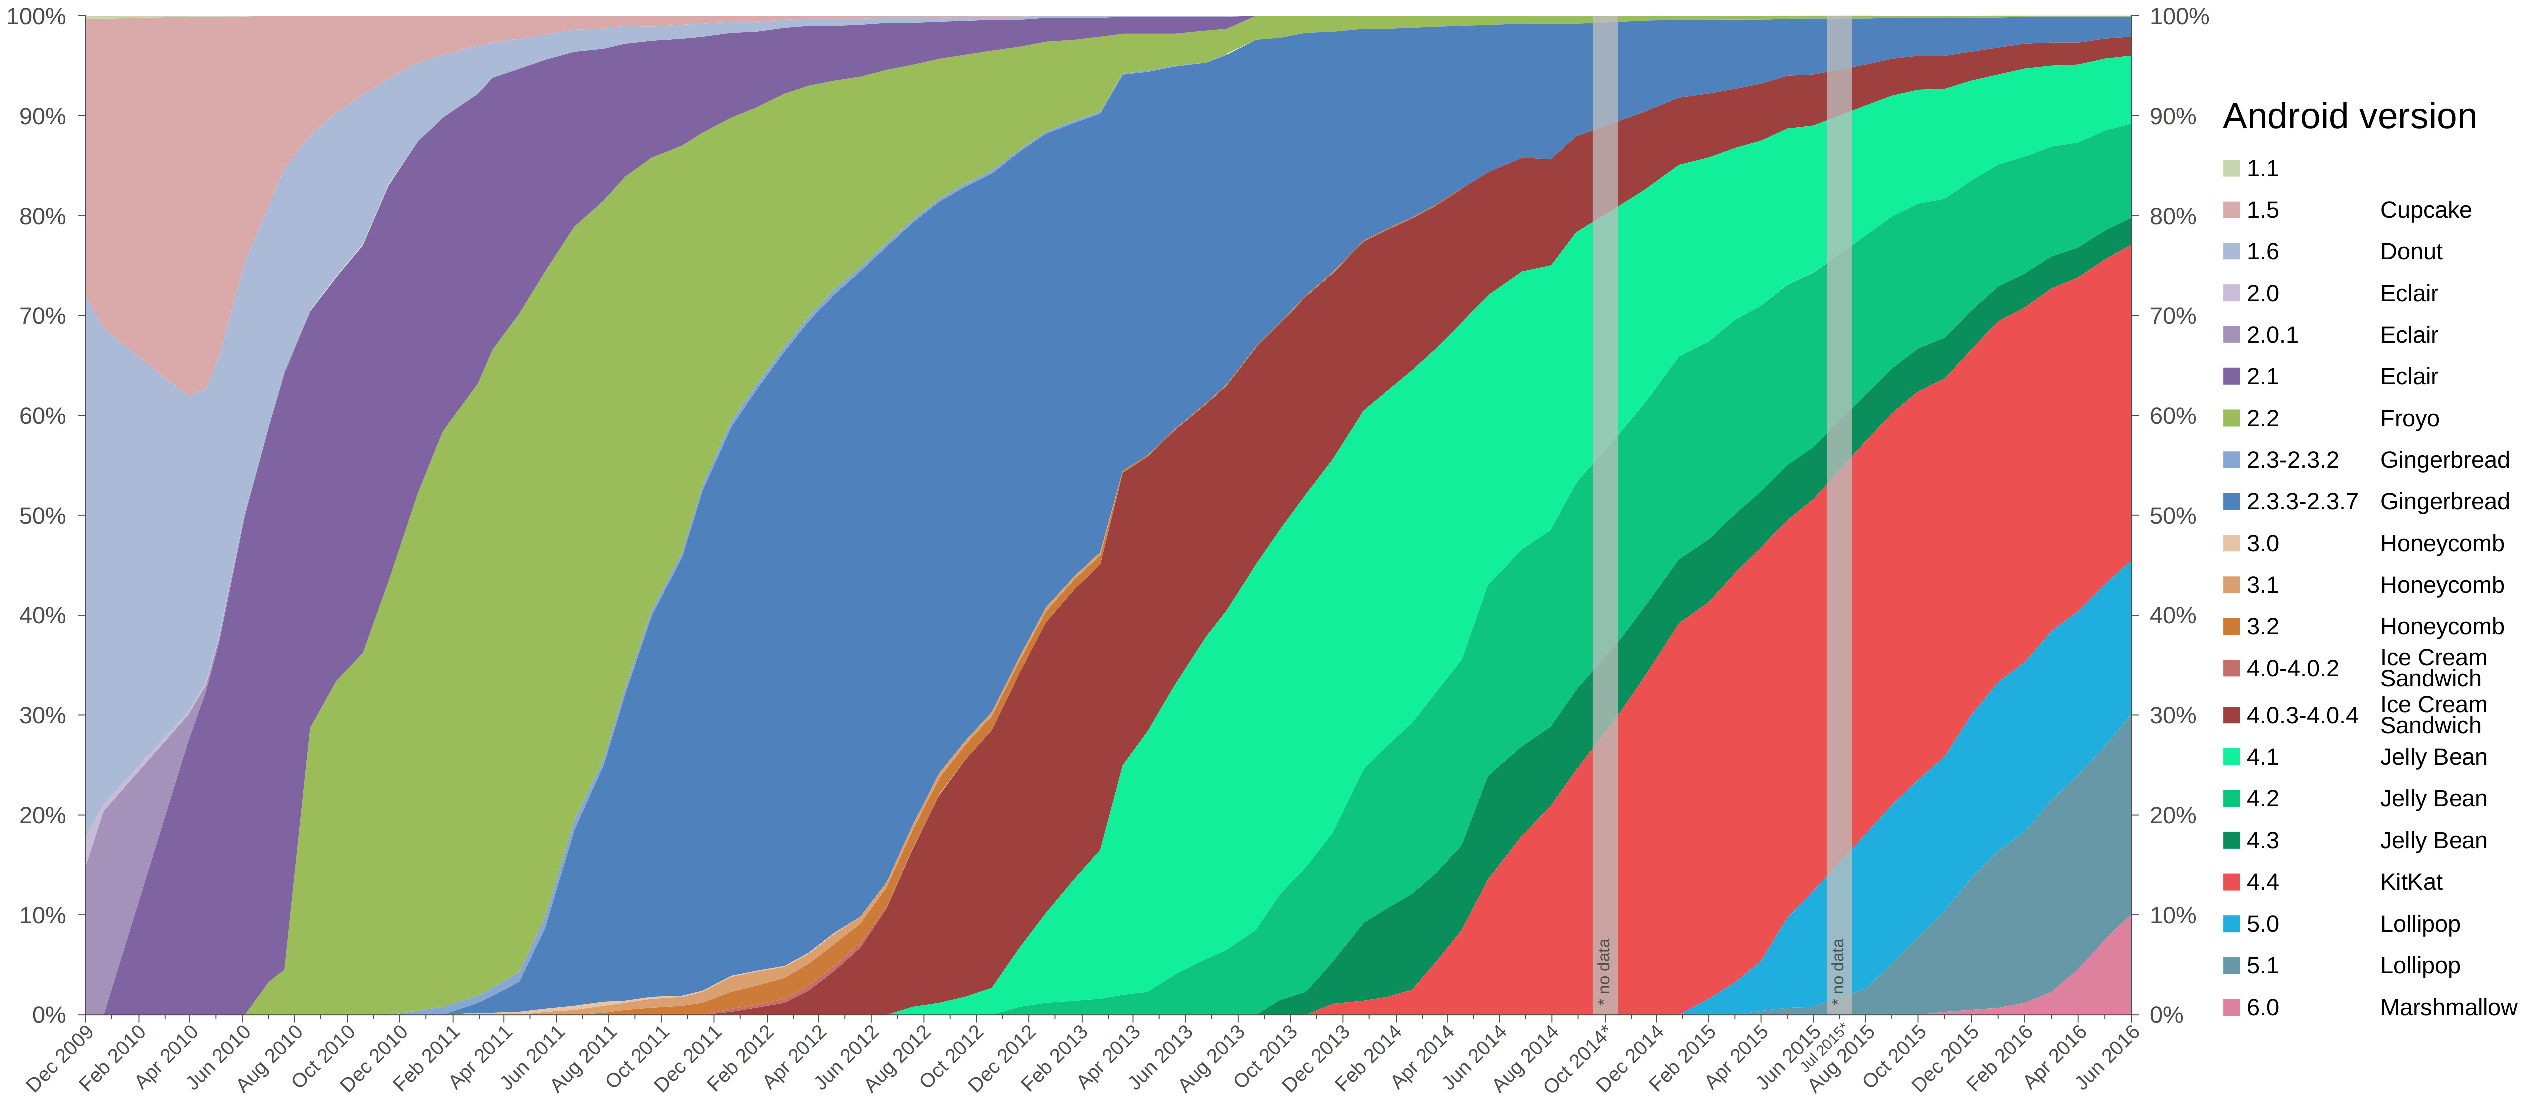
\includegraphics[width=\linewidth]{figures/android-versions.pdf}
\caption[Historical Android version's distribution.]{Historical Android
  version's distribution~\cite{erikrespo_android_2017}.}
\label{fig:android-versions}
\end{figure}

Mobile devices became more ubiquitous, and \acp{PDA} reappeared now
called \emph{tablets} or \emph{iPads}.  These devices were identical
to the smart phones, but larger and they generally did not have a
cellular data connection instead using wifi. They could not send
texts or make phone calls but a shift away from traditional SMS and
cellular phone calls to internet backed communications such as
WhatsApp, iMessage, Skype and FaceTime meant these devices were
essentially interchangeable with smart phones.

Advances in secure co-processors meant that mobile devices were even
more capable.  Banks allowed users to link their devices to their bank
accounts and use their device, or even the new \emph{smart watches} as
a debit card.  This quickly became a common and ubiquitous payment
method quickly with even street vendors, who hadn't taken cards
previously, accepting contactless payment via a mobile device.  The
separation of cryptographic operations from everyday computing with
secure co-processors and secure enclaves (such as TrustZone) lead to
significantly improved security.  Keys could be isolated from the
entire mobile OS, allowing for increased trust mechanisms.

Mobile devices gained the ability to collect increasingly personal
information.  Smart watches recorded and shared a user's pulse with
others. Mobile health apps were made to track and monitor medical
conditions. In the US, the \ac{HIPAA} required that healthcare
providers transmited medical information securely, but many apps had
basic security problems~\cite{fahl_why_2012}, and many of the
healthcare apps did not handle the medical information
securely~\cite{knorr_privacy_2015}.

\subsection{App Stores}

%\todo{Introduce how app stores are the primary mechanism for
%distributing software in the ecosystem.  Describe and possibly show
%the interface, and reviews.  Maybe move the marketshare diagram from
%later on into here?  }

The app store has become the normal method for distributing software
on mobile devices.  These stores run as apps on the device and show
lists of software that the user can install on their device.  Users
can browse, buy apps or install free versions, or read and leave
reviews.  To install an app on an early mobile device the user would
download it on a traditional computer and then transfer it to the
mobile, where they could install it using a package manager.  App
stores considerably streamlined this process, allowing users to find
an install apps straight from their device.  Whilst the app store is
the normal method of installing apps, apps can still be downloaded and
installed manually by side-loading on Android or through iTunes for
iOS.

\begin{figure}
  \centering
  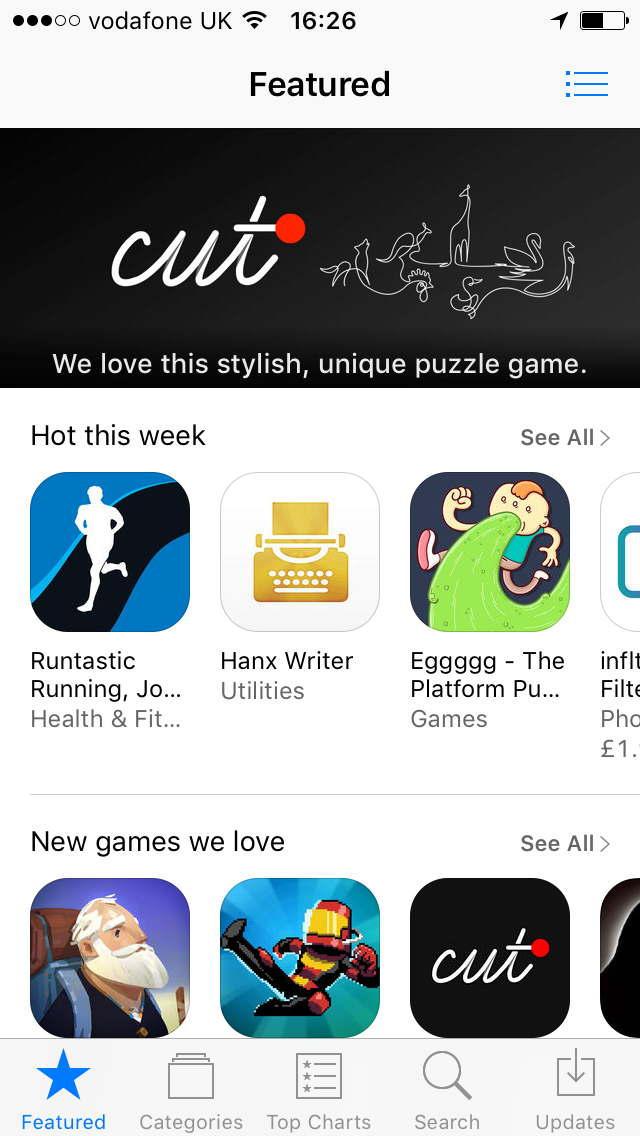
\includegraphics[width=0.31\textwidth]{figures/store-home.png}
  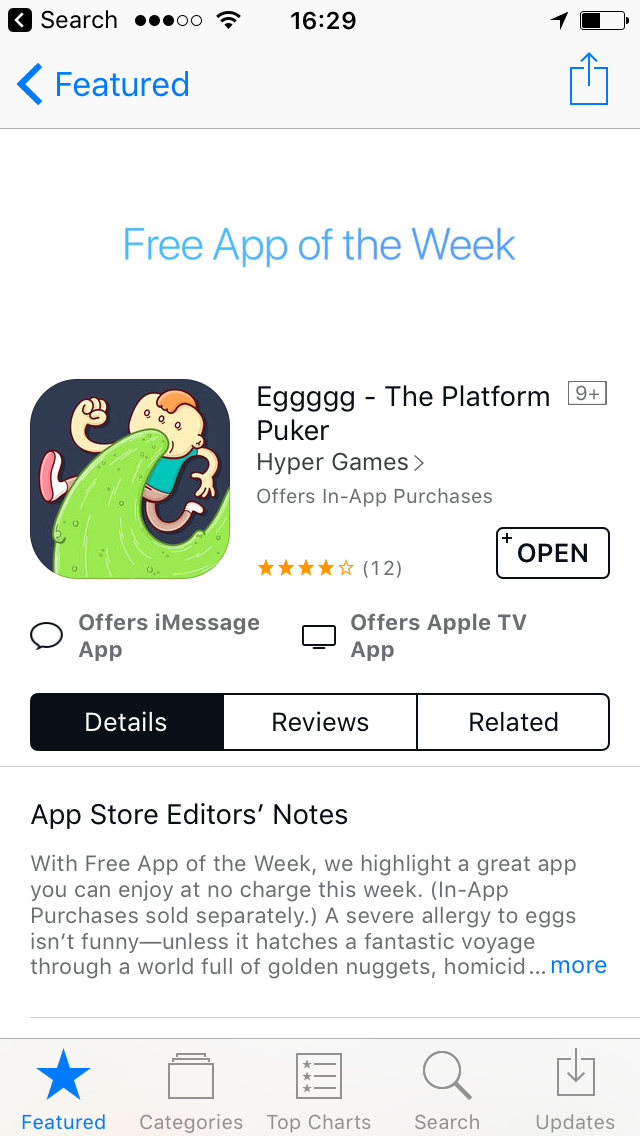
\includegraphics[width=0.31\textwidth]{figures/store-app.png}
  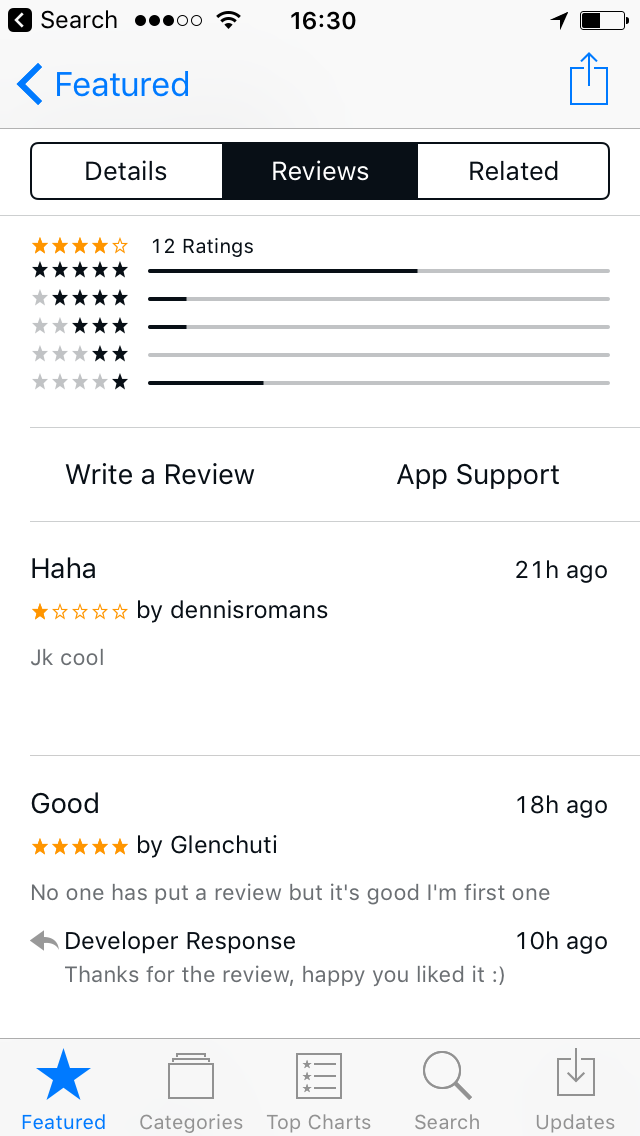
\includegraphics[width=0.31\textwidth]{figures/store-review.png}
  \caption[Apple's App Store.]{Apple's App Store.  Showing the store's frontpage, an app's page, and its reviews.}
  \label{fig:appstore}
\end{figure}

Figure~\ref{fig:appstore} shows Apple's App Store.  Users are first
presented with featured apps, though they can also browse for apps by
category, search, or look at \emph{top charts}.  If a user touches an
app they are presented with more information.  This particular app,
\emph{Eggggg}, is the free app of the week.  The app's name and
age-rating (9+) is shown alongside the a link to the app's developer.
A button is presented for the user to install the app or open it if it
has already been opened.  Additional information is displayed about
the app: it will work with Apple's messaging app, and also with their
Apple TV devices.  The App store editor has, in this case, written a
note about it describing the app which is displayed prominently.  If
the user reads down the page a description of the app by the developer
is also given, as well as screenshots, a changelog, detailed
information including device compatibility, and a link to the apps
privacy policy.  This particular app offers in app purchases and the
user is warned of this prominently on this screen.  A review score is
also displayed. This app has 4 out of 5 stars based on twelve reviews.
If the user touches the review tab, they can see more detailed reviews
by named reviewers.  These can vary in quality (this particular app's
top reviews are not helpful) and the developer can respond to
individual reviews.  User's can optionally write a review for the app.

Whilst Apple and Google's app stores are the largest, others are also
available.  On Android, whilst Google's Play Store is often the
default, users are free to choose other marketplaces if they wish.
One choice is Amazon's Appstore.  It is the default for Amazon's
Kindle Fire tablets, and has special offers for Amazon customers.
Other marketplaces are regional.  In China, where Google web services
cannot be used, alternative markets such as Qihoo360 and Baidu have
sprung up.

Precise numbers of apps in different stores is hard to get, but the
largest stores occassionally give rough
numbers~(\autoref{fig:app-store-apps}).  Google and Apple's stores
have (as of the end of 2016) around 2.5 million apps, with Amazon's
store having considerably less.

\begin{figure}
  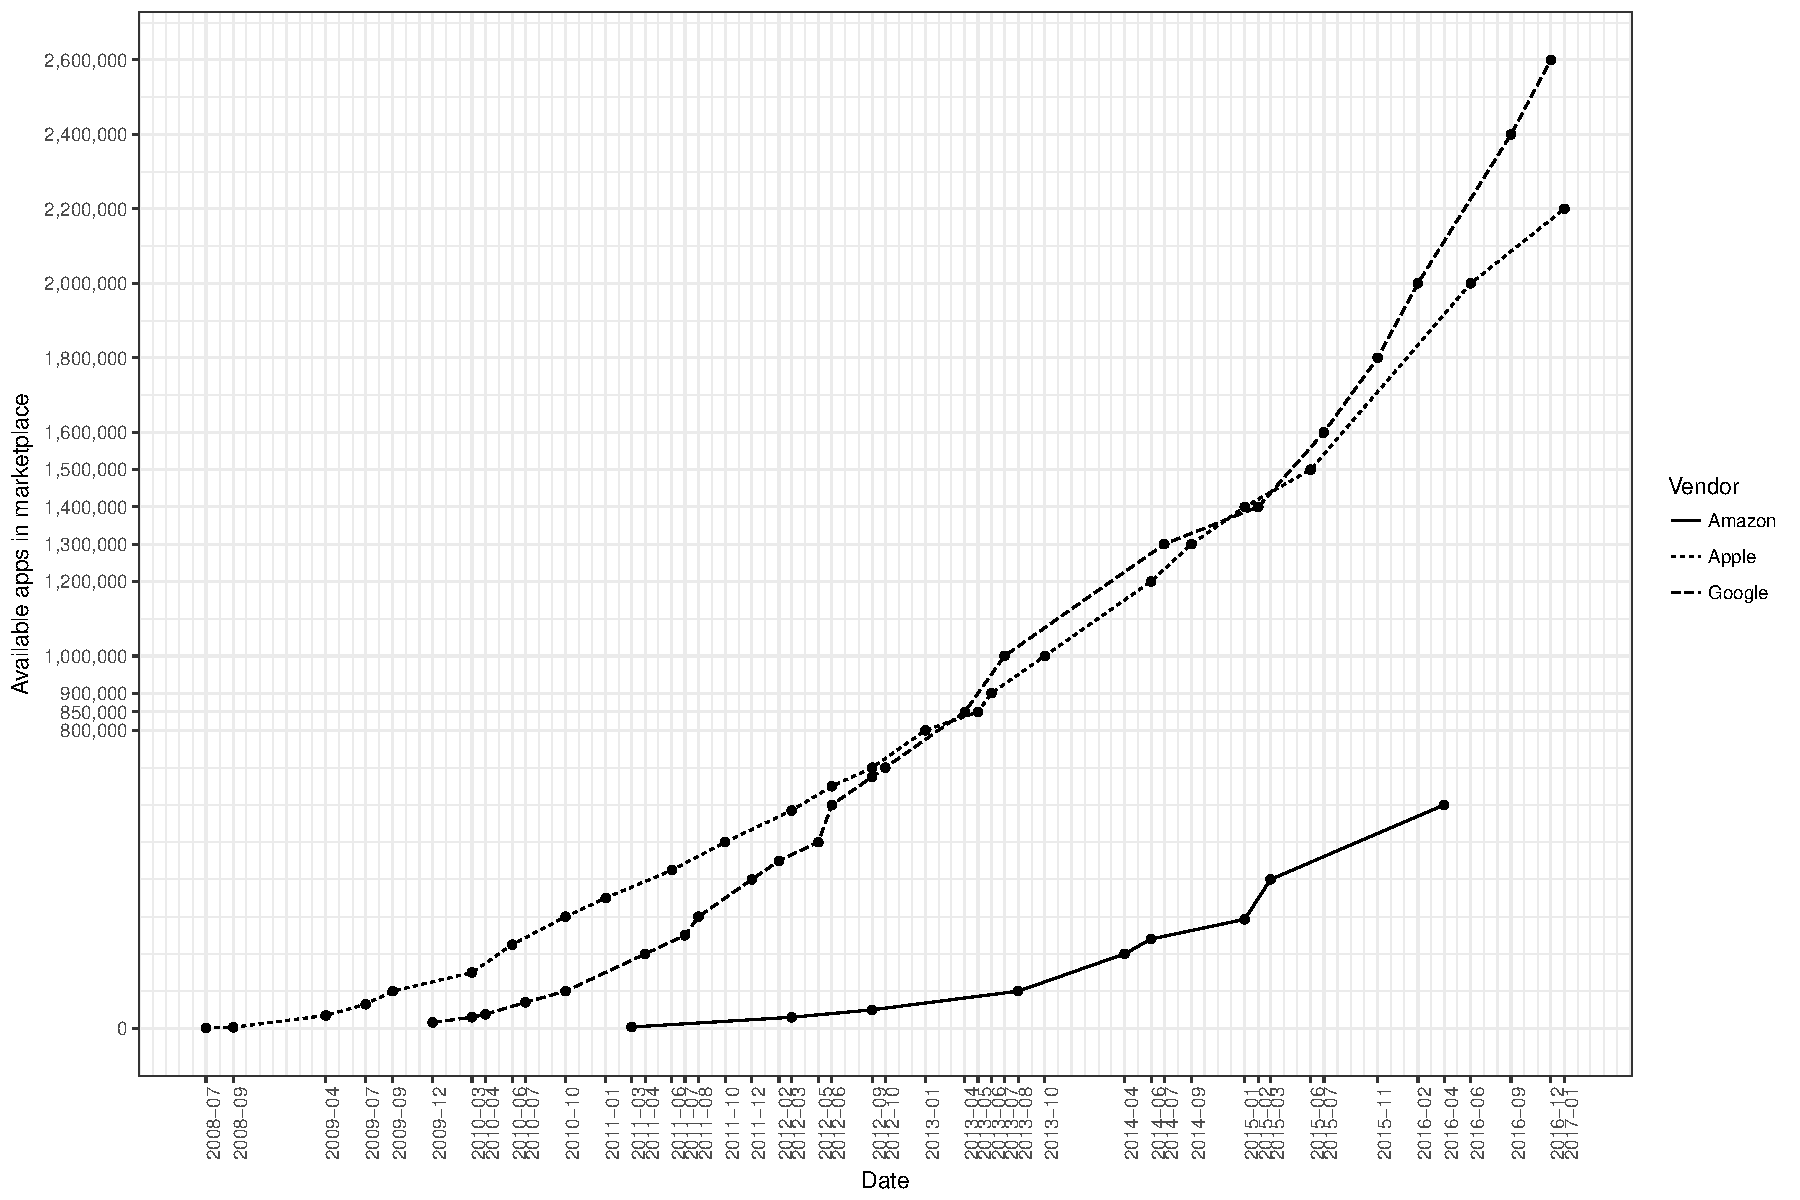
\includegraphics[width=\textwidth]{figures/app-store-apps.pdf}
  \caption[Reported numbers of different apps on various App marketplaces.]{%
    Reported numbers of different apps on various App marketplaces. Data taken from~\cite{statista_google_nodate,statista_apple_nodate,statista_amazon_nodate}.}
  \label{fig:app-store-apps}
\end{figure}

Each of these different stores have different terms and conditions,
and different criteria for developers to sell their apps in.  These
are written in long, dense, legal documents. We will return to these
documents in \autoref{chap:apps-and-app-stores} when we make a
comparison between them.

Apple's devices are limited normally only have access to Apple's App
Store; however there is a second, unofficial, method of installing
apps.  Jay Freeman's \emph{Cydia} is an alternative method for
installing apps on jailbroken devices.  When a jailbreak is released
they usually install the Cydia store as well.  Cydia itself is build
atop of Debian's \emph{dpkg} framework and relies on various
\emph{repositories} for hosting and distributing the apps.

Anyone is free to host their own repository but often the
\emph{``official''} repository is \emph{BigBoss}.  BigBoss is further
split into three stores: free, CydiaStore with purchases handled by
the Cydia store, and CydiaStore with purchases handled by the app and
their own payment mechanisms.  To host an app in their store they list
only 5 conditions~\cite{bigboss_host_2014}.

\begin{quotation}\noindent
  \begin{enumerate}
    \item You must own the app and be the developer of the content

    \item No porn or adult apps. No swagbucks style apps where user
      makes you money by shopping with your ID.

    \item You can only use one Cydia repository. If you submit here do
      not submit this to another major host elsewhere or it will have to be
      removed from one of the repositories. (You can host this in your own,
      private repository still just not any other major community
      source). There is no benefit to having duplicate packages in major
      sources as you get the same exposure by using just one.

    \item Screenshots for any GUI app are required. If you don't
      provide screenshots, your submission will be delayed.

    \item Make sure your app is signed with \emph{ldid}\footnote{A
        tool for jailbroken devices that generates SHA-1 hashes that iOS
        checks for in all code~\cite{saurik_code_nodate}.} and properly
      built. We recommend you build with Theos but you can use whatever you
      want as long as you test in a jailbroken iOS enviornment. Thie means
      you should not be submitting xcode generated IPA files as this is a
      dead giveaway that you did not test properly.
  \end{enumerate}
\end{quotation}

The Cydia based stores are considerably less formal than the Android
marketplaces, and they require less information and have fewer terms.
There are several explanations for this: enthusiasts run the stores
not companies, they rely upon having root access to the OS which is
prohibited by Apple.  In this thesis we are not going to consider
these stores as they are, by necessity, outside of the scope of the
standard mobile ecosystems.  They are, however, worth mentioning for
the sake of completeness.

%The other iOS stores worth mentioning (though again we will not
%consider them) are the piracy stores.  These exist to allow users to
%download pirated paid apps from the App Store without paying.  Perhaps
%the most notable of these was the \emph{Installous} Cydia repo which
%hosted pirated apps for many years.  These stores come and go as they
%are shutdown; some working through Cydia, and some offering pirated
%\emph{IPA}s (Apple's app package format) for installation through
%iTunes.  Again, we will not cover these stores (in part because they
%are so transient) but they are worth mentioning as they represent part
%of the mobile ecosystem that a minority of Apple's users use, that is
%more open than the marketplace Apple provide.

\subsection{The Need For Policies}

With mobile devices becoming increasingly capable and holding
ever-increasing amounts of information there is a need from users and
businesses to manage how the devices behave.  Employees now bring
their mobile devices to work and use them to access company email and
documents.  In response to this companies publish mobile device
policies that describe how the devices should be used within the
company.  These policies vary in terms of formality.  A user may never
write their privacy preferences in a formal language, but they may
make decisions guided by them.  For example which apps to install and
which to avoid.  They may make decisions based on what their friends
have told them, or what a review said about the app.  They may also
use \ac{MDM} software to enforce the policies.  If a company wishes to
use an app for business purposes there may be regulation they need to
follow, such as \ac{HIPAA}.

A company looking to control the mobile devices their employees bring
to work might write a \ac{BYOD} policy.  They might also use \ac{MDM}
software to control some aspects of their devices.  The company might
write these with varying degrees of formality but often they are
written using natural language.  This adds vagueness and can lead to
confusion as to how a policy should be implemented.  By describing the
policy in a formal language we can start to express the policy more
rigorously.  We can start to make comparisons between users, and with
rules for checking the policy start to help the user to make decisions
more accurately, or measure the extent a user follows their stated
policy.  Using formal languages we can
model the policies precisely, helping clarify their meanings and make
precise comparisons between different policies.  We can tie the rules
in the \ac{BYOD} policies, for example, to the \ac{MDM} tools used to
implement them.

If a company needs to use apps which conform with a policy such as
\ac{HIPAA} they could use static analysis tools to check for some
aspects of the policy.  Perhaps the company might use
Mallodroid~\cite{fahl_why_2012} to detect when data is sent
unencrypted.  It is important, however, not to confuse the tools and
techniques we might use to implement parts of a policy with the end
goal of ensuring that the policy is followed.  A formal language that
lets us sever the policy from its implementation can help us
understand the policy precisely, and then show precisely how the
policy is checked.  It lets us see what rules from the policy are
checked for by which tools, and identify gaps where the policy is not
being checked sufficiently.

A key aspect of the mobile ecosystem is delegation.  The user of a
mobile device (typically) first logs on to a Google or Apple account
before using the device, which retrieves all their data.  Even in an
app rather than store all the data locally the app may prompt the user
to log in and delegate to a third-party (such as Google or Facebook)
to manage the account ID.

Users may install apps manually themselves, but they might use one or
more app stores to provide them with apps.  They trust these app
stores to provide them with \emph{good and safe} apps, and delegate
the checking of them to the store.  Whereas a user might once have
done the check themselves (or at least delegated to an \ac{AV} package
on their computer) now the responsibility is handed to the stores.
Furthermore all software comes signed either by the developer who
created it (in the case of Google's Play Store), the store that sold
it (in the case of Amazon's app store) or both (Apple's App Store).  A
store may delegate to a third-party app vetting service to determine
what apps are safe (Yandex and Aptoide stores), or use their own
in-house teams.

On Android there is a requirement that whenever
an app is updated the update's signature must be from the same key as
the app it is updating.  This means that there is a delegation from
the OS to the developer to say what is a valid update, but also a
trust relationship from the user to the developer (or store) to
provide updates at all, as no-one else will be able to patch the
software.

Users recommend each other apps.  Some may consider what apps they
want to use on their phone and come up with internalized policies that
describe how they want to use them, and may trust reviews to give them
an idea of an app's quality, and the phone itself to tell them what
functionality the app has through its permissions.

They allow their employers to say how they should their devices, who
may in turn delegate to IT departments, to write rules, which may
delegate back to the users to state what rules they're willing to
follow.

These trust relationships and delegations permeate the entire mobile
ecosystem.  They represent an important aspect of the ecosystem that a
policy language should catch in order to adequately describe the
relationships and policies within it.


%When describing how mobile phones had evolved, we described how we
%arrived with two main operating systems for mobile devices: iOS and
%Android.  The trust models in the systems differ, as do the
%assumptions about what an app can do when running on each system.
%There are also similarities.  iOS and Android (from Android M) have a
%similar permissions system for apps.  When people make comparisons
%between them, however, the differences are often vague.  iOS is a
%\emph{walled garden}.  Android is \emph{more open}.  Again, by using
%formal languages we can start to make comparisons that are precise and
%show the differences clearly.

% I'm a bit unsure about this...
One approach to designing a policy language is to base it on a logic
of authorization.  These authorization logics describe rules for
deciding when an action is permitted, and reasoning about why that
action was allowed.  A common use case for these logics is building
access control systems: users are allowed to read a file if they have
the appropriate permissions.  In applying logics of authorization to
policy language the policy language describes who can access what, but
the authorization logic gives a formal description of how we make that
decision.

We need an authorization language for mobile ecosystems.

\section{SecPAL}

SecPAL is an authorization language developed by Becker~\etal~to
describe policies and delegation chains surrounding distributed
services~\cite{becker_secpal:_2010}. It was designed as a high-level
human-readable language that allowed the policy specification and
maintenance to be separated from the implementation mechanisms.

SecPAL was designed to improve over previous high-level languages in
several areas.  It was designed to be more expressive than
XrML~\cite{kolovski_logic-based_2007},
SPKI/SDSI~\cite{ellison_spki_1999}, and Delegation
Logic~\cite{li_delegation_2003}; and more readable than
XACML~\cite{oasis_extensible_2013} and other XML-based policy
languages.  Furthermore it was designed to be intuitive and
unambiguous with precise semantics unlike other languages (most notably
XACML) which had natural language descriptions with ambiguous and
inconsistent specifications that had been retrofitted to the language
instead of being designed with the language in the first
place~\cite{bryans_reasoning_2005,ramli_logic_2014,masi_formalisation_2012}.

SecPAL's original application was to model and enforce access control
policies in grid computing systems~\cite{becker_secpal:_2010}.  In
this dissertation we describe how the language can be extended to
describe the policies surrounding the mobile ecosystem.

At its core, SecPAL is a language with a simple grammar
(\autoref{fig:secpal-grammar}) and three evaluation rules
(\autoref{fig:secpal-rules}). The language's simplicity makes it easy
to apply to a new domain by instantiating it with predicates and
constraints that describe the domain. This simplicity does not come at
the cost of its expressiveness. SecPAL supports delegation (by using
\emph{can-say} verbs), role and attribute based policies (by using
\emph{can-act-as} verbs) and arbitrary constraints.

\begin{figure}
  \newcommand{\bracetext}[1]{\text{\sffamily #1}}
  \newcommand{\smalltext}[1]{\text{\ttfamily\small #1}}
  \centering
  \begin{equation*}
    \begin{array}{r l}
      \overbrace{\smalltext{`user'}}^{\bracetext{speaker}} &
                                                             \smalltext{ says }\overbrace{\overbrace{\smalltext{ App }}^{\bracetext{subject}}\overbrace{\smalltext{ isRunnable}}^{\bracetext{predicate}}}^{\bracetext{fact}} \\
                                                           & \overbrace{\smalltext{ if App isFree}}^{\bracetext{condition}} \\
                                                           & \overbrace{\smalltext{ where hasPermission(App, `INTERNET') = true}}^{\bracetext{constraint}}.
    \end{array}
  \end{equation*}
  \caption{Structure of a SecPAL assertion.}
  \label{fig:assertion}
\end{figure}

\newcommand{\bnfcomment}[1]{\slshape{\sffamily(#1)}}
\newcommand{\secpal}[1]{\texttt{#1}}
\begin{figure}\footnotesize\centering
  \begin{tabular}{r r l c}
    AC         & $\Coloneqq$ & assertion$_1$ \dots assertion$_n$                      & \bnfcomment{assertion context} \\
    assertion  & $\Coloneqq$ & e \secpal{says} claim.                          \\
    e          & $\Coloneqq$ & \secpal{x}                                       & \bnfcomment{variables}         \\
               & $\vert$     & \secpal{A}                                       & \bnfcomment{constants}         \\
    predicate  & $\Coloneqq$ & \secpal{has} $\vert$ \secpal{can} $\vert$ \dots  & \bnfcomment{predicates}        \\
    D          & $\Coloneqq$ & 0                                                & \bnfcomment{no delegation}     \\
               & $\vert$     & $\infty$                                         & \bnfcomment{unbounded delegation}        \\
    vp         & $\Coloneqq$ & predicate e$_1$ \dots e$_n$                           & \bnfcomment{verb phrase}       \\
               & $\vert$     & \secpal{can-say}$_D$ fact                       \\
               & $\vert$     & \secpal{can-act-as}  e                          \\
    f          & $\Coloneqq$ & e vp                                             & \bnfcomment{fact}              \\
    claim      & $\Coloneqq$ & f \secpal{if} f$_1$,\dots, f$_n$; c             \\
    c          & $\Coloneqq$ & $\top$                                           & \bnfcomment{no constraint}     \\
               & $\vert$     & e$^\prime_1 =$ e$^\prime_2$                      & \bnfcomment{constraints}       \\
               & $\vert$     & \dots                                           \\
    e$^\prime$ & $\Coloneqq$ & e $\vert$ function(e$_1$,\dots e$_n$)           \\
  \end{tabular}
  \caption{BNF description of SecPAL.}
  \label{fig:secpal-grammar}
\end{figure}

%Other domains have successfully used
%variants of SecPAL to describe their policies. Humphrey~\etal{}
%instantiated SecPAL with predicates for the GridFTP protocol to create
%a Grid access control policy
%language~\cite{humphrey_fine-grained_2007}. Aziz~\etal{} created
%SecPAL4DSA by adding predicates for data-sharing
%agreements~\cite{aziz_secpal4dsa:_2011}.  Becker~\etal{} added
%predicates for describing \ac{PII}-handling preferences and created
%SecPAL4P~\cite{becker_framework_2009}.


\begin{figure}
  \footnotesize\centering
  \renewcommand{\says}[1]{\text{says}}
  \renewcommand{\AC}[0]{\text{AC}}
  \renewcommand{\canSay}[1]{\text{can-say}_{\text{#1}}}
  \renewcommand{\canActAs}[0]{\text{can-act-as}}
  \renewcommand{\where}[0]{\text{where}}
  \begin{equation*}
    \infer[\text{cond}]{
      \AC{}, D \models A~\says{\bigoplus_{i=1}^n p_i}~f\theta
    }{
      \begin{matrix}{
          \left(A~\says{}~f~if~f_1\cdots f_n~\where~c\right) \in \AC{}
        }\\{
          \forall i \in [1\cdots n]. \AC{}, D \models A~\says{}~f_i\theta
        }
      \end{matrix}&
      \vdash c\theta &
      vars\left(f\theta\right) = \emptyset
    }
  \end{equation*}
  \begin{equation*}
    \infer[\text{can-say}]{
      \AC{}, \infty \models A~\says{p_1 \oplus p_2}~f
    }{
      \AC{}, \infty \models A~\says{p_1}~B~\canSay{D}~f &
      \AC{}, D \models B~\says{p_2}~f
    }
  \end{equation*}
  \begin{equation*}
    \infer[\text{can-act-as}]{
      \AC{}, D \models A~\says{p_1 \oplus p_2}~x~vp
    }{
      \AC{}, D \models A~\says{p_1}~x~\canActAs~y &
      \AC{}, D \models B~\says{p_2}~y~vp
    }
  \end{equation*}
  \caption{SecPAL's evaluation rules.}
  \label{fig:secpal-rules}
\end{figure}


\begin{figure}\centering\sffamily\footnotesize
  \begin{tabular}{c l p{0.6\linewidth}}
    \toprule
    \multirow{3}{*}{\rotatebox{90}{Concepts\hspace{1em}}} & $AC,\theta \vdash q$                     & Defining relation. A query assertion $q$ is valid given the assertions contained in the assertion context $AC$ and a variable substitution $\theta$. \\
    &$\epsilon$                               & The empty substitution. \\
    
    \midrule
    \multirow{5}{*}{\rotatebox{90}{Definitions}} &
    1. $AC,\theta \vdash \overbrace{e \text{ says } fact}^q.$  & if $AC,\infty \models e\theta \text{ says } fact\theta$ and $dom(\theta) \subseteq vars(e \text{ says } fact)$                                       \\
    &2. $AC,\theta_1\theta_2 \vdash q_1, q_2$    & if $AC,\theta_1 \vdash q_1$ and $AC,\theta_2 \vdash_2 q_2\theta_1$                                                                                   \\
    &3. $AC,\theta \vdash q_1 \text{ or } q_2$   & if $AC,\theta \vdash q_1$ or $AC,\theta \vdash q_2$                                                                                                  \\
    &4. $AC,\epsilon \vdash \mathsf{not}(q)$     & if $AC,\epsilon \not\vdash q$ and $vars(q) = \emptyset$                                                                                              \\
    &5. $AC,\epsilon \vdash c$                   & if $\models c$                                                                                                                                       \\
    \bottomrule                             \\
  \end{tabular}
  \caption[SecPAL's semantics.]{SecPAL's semantics as described by Becker~\cite{becker_secpal:_2010}.}
  \label{fig:secpal-semantics}
\end{figure}

SecPAL's semantics are given in \autoref{fig:secpal-semantics}.  A
query $q$ to a SecPAL program (which is a collection of facts and
relationships called the \emph{assertion context} or \emph{AC}) asks
if there exists a renaming $\theta$ such that the rules of SecPAL can
be used to derive the, possibly renamed, query ($AC,\theta \vdash q$
if $AC,\infty \models q\theta$)\footnote{$\vdash$ describes if a query
  is valid with respect to an AC, whereas $\models$ says there is a
  valid proof for a SecPAL using the rules of SecPAL.  Conjugation,
  disjunction and negation are allowed within a query, but not when
  evaluating SecPAL.}.  The renaming must be specific and talk only of
the variables contained in the query, conjunction and disjunction work
as expected.  Negation is only allowed in an extremely limited form: a
query can be not true if it contains no variables and there is no way
to show that the AC supports the query.  This limited form means that
queries remain decidable: the rules inside the AC are not permitted to
use negation.

A key feature of SecPAL is the ability to delegate statements.  SecPAL
was designed to make access control decisions over large networks.
Rather than have a centralized decision server where all decisions are
made, SecPAL allows information to be shared through assertions signed
by their speaker.  This allows different principals to be responsible for different decisions and make decisions independently.
An example of this, expanded from one given by Becker~\cite{becker_secpal:_2010}, is of a researcher attempting to run a query on a cluster, using data from a fileserver (\autoref{fig:delegation-example}).

\begin{figure}
  \centering
  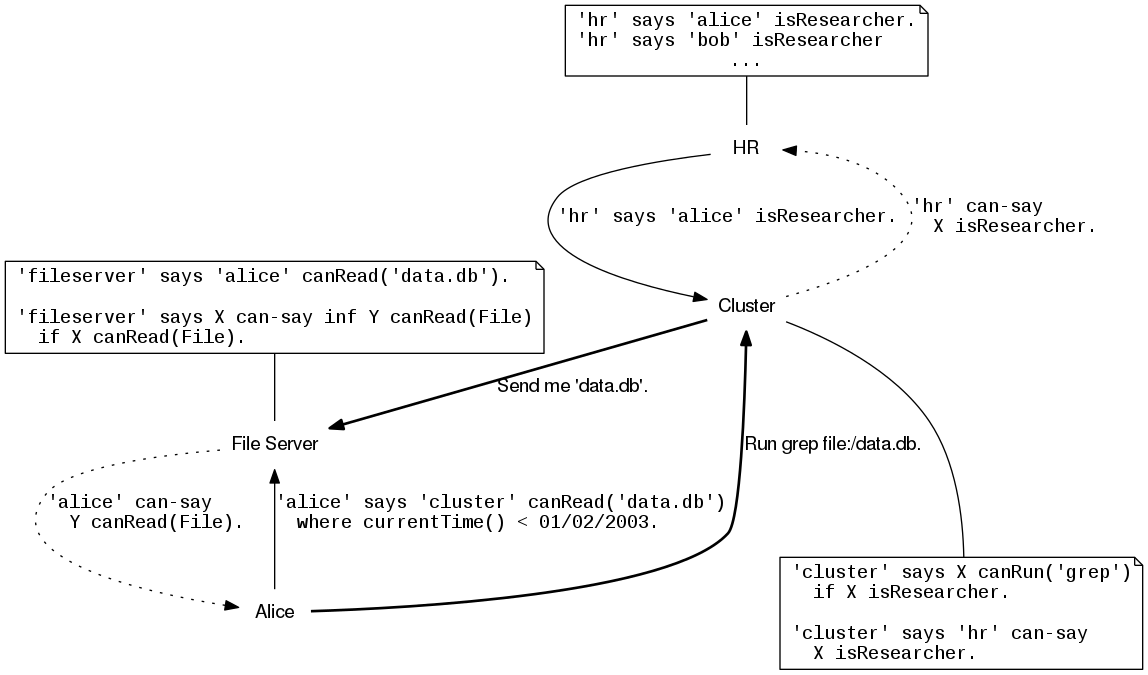
\includegraphics[width=\textwidth]{figures/secpal-example.png}
  \caption[Example of delegation on a cluster.]{Example of delegation when running a command on a cluster.  Bold links show requests, plain links show the sending of SecPAL statements, and dotted links indicate delegation relationships.  SecPAL assertions at each location are shown in notes.}
  \label{fig:delegation-example}
\end{figure}

Alice sends a request to the cluster to run a search on her data on the file-server.
The cluster has a SecPAL policy that only researchers can run the search:
\begin{lstlisting}
'cluster' says X canRun('grep')
  if X isResearcher.
\end{lstlisting}
and a rule that says only HR can say who is a researcher or not.
\begin{lstlisting}
'cluster says 'hr' can-say
  X isResearcher.
\end{lstlisting}
The cluster queries HR if Alice is a researcher or not and HR responds by sending the assertion that she is.
\begin{lstlisting}
'hr' says 'alice' isResearcher.
\end{lstlisting}
The cluster does not know how HR knows that Alice is a researcher, but
is content with HR's assertion that she is.  HR may have a SecPAL
instance and policy of their own to make this and send it to the
cluster, or they might be using a conventional database.  Provided
they give this signed SecPAL assertion to the cluster, it doesn't care
how they came by it.  The one limitation the cluster has is that it
\emph{must} be HR who tells them; HR cannot delegate the decision
further.

With the cluster convinced that Alice is authorized to run the search,
the cluster requests the database from the file server.  The file
server knows that Alice can read her data and that anyone who can read
a file is permitted to say who else can read it.
\begin{lstlisting}
'fileserver' says 'alice' canRead('data.db').
'fileserver' says X can-say inf Y canRead(File)
  if X canRead(File).
\end{lstlisting}
Using SecPAL, the file server, determines that Alice can say who can
read her data.  Alice provides the file server with a statement that
the cluster is authorized to read her file (for a short time
period).
\begin{lstlisting}
'alice says 'cluster' canRead('data.db')
  where currentTime() < 01/02/2003.
\end{lstlisting}
Dutifully the file server provides the cluster with the data
it required.  The cluster runs the search and hands the results back to Alice.

\begin{figure}
  \centering
  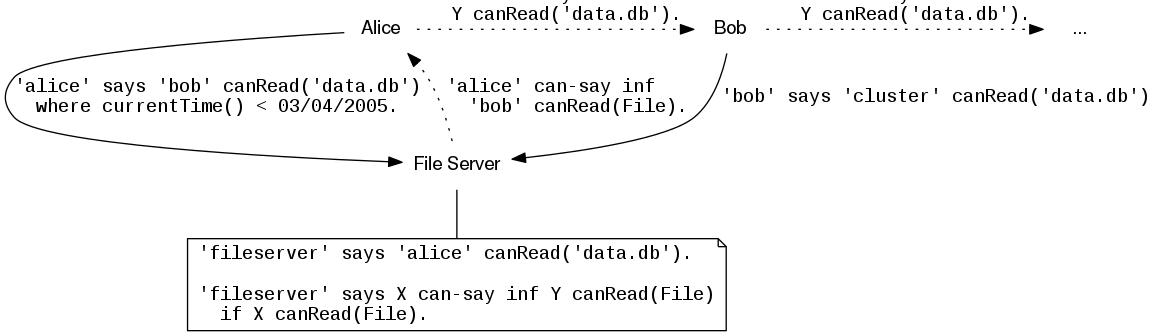
\includegraphics[width=\textwidth]{figures/secpal-example-delegation.png}
  \caption{Example of unbounded delegation.}
  \label{fig:unbounded-example}
\end{figure}

This simple example shows how different principals can make decisions using delegation mechanisms, and by sharing assertions.
SecPAL allows for more complicated delegation relationships, however. When checking who could access Alice's data, the file server allowed Alice the ability to delegate the decision of who could read her file by using the \texttt{can-say inf} verb.
Alice might allow Bob to share her data set with others who might also be allowed to share it for a limited time (\autoref{fig:unbounded-example}).

\begin{figure}
  \centering
  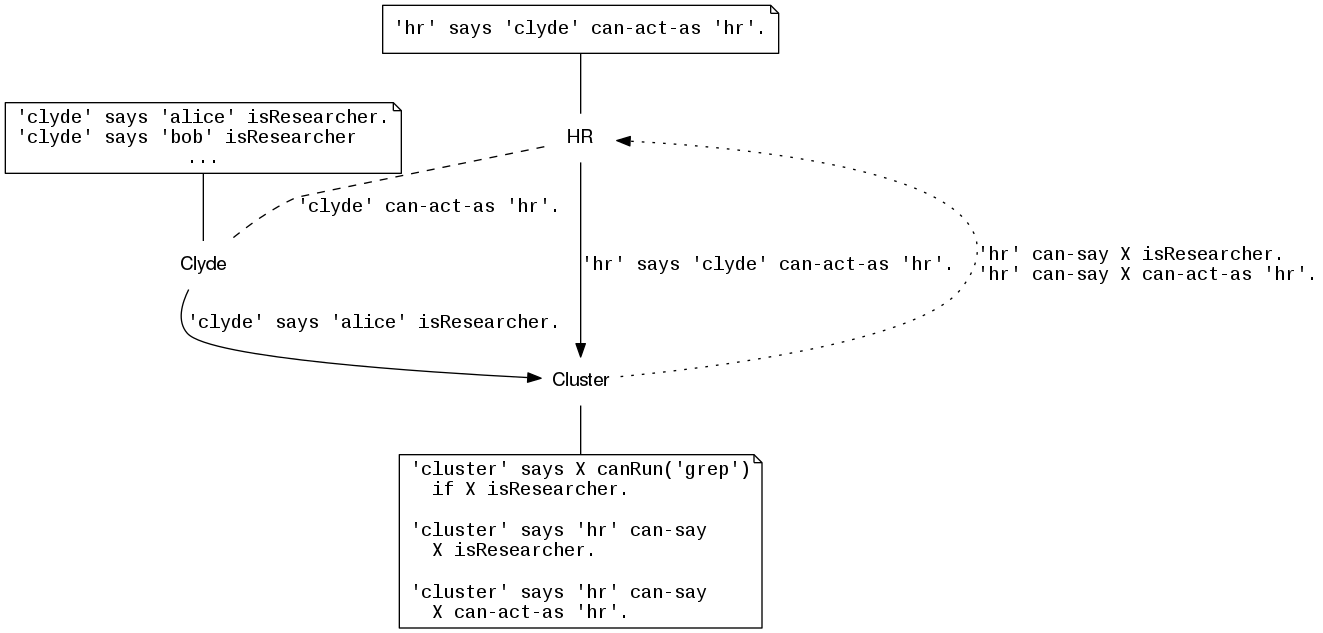
\includegraphics[width=\textwidth]{figures/secpal-example-roles.png}
  \caption[Example of delegation with roles.]{Example of delegation with roles.  Role relationships are shown with dashed links.}
  \label{fig:roles-example}
\end{figure}

An alternative to the delegation to the HR server to determine if
Alice was a researcher would be to use delegation with roles (shown in
\autoref{fig:roles-example}).  HR may consist of many principals.  The
cluster may be happy to accept the word of anyone who works in HR as
if they were HR.  To do this the cluster adds a delegation to HR that
they can name anyone who acts as them, and HR respond by saying that
Clyde can act for them.
\begin{lstlisting}
'cluster' says 'hr' can-say
  X can-act-as 'hr'.
'hr' says 'clyde' can-act-as 'hr'.
\end{lstlisting}
Now on the cluster Clyde's word is as good as HR's.
Clyde sends the necessary facts about Alice and the program can be run as before.
It is important to note that any restrictions on HR also apply to Clyde.  He still cannot delegate the decision further.

\begin{figure}
  \centering
  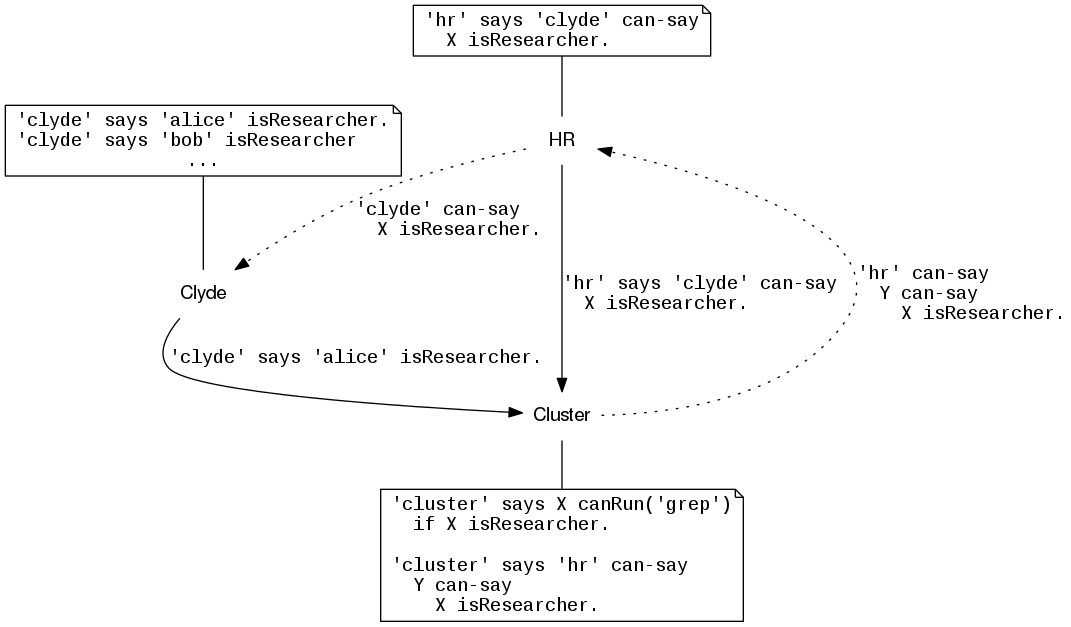
\includegraphics[width=\textwidth]{figures/secpal-example-delegation2.png}
  \caption{Example of depth bounded delegation.}
  \label{fig:depth-example}
\end{figure}

As an alternative to roles, depth-bounded delegation with the
\emph{can-say} statement could also have been used
(\autoref{fig:depth-example}).  In this case instead of delegating the
decision of who is a researcher to HR, the cluster delegates the
\emph{decision of who can make the decision} to HR.  HR makes the
delegation to Clyde, and the process continues as before.
Depth-bounded delegation allows delegation statements to be chained to
an arbitrary (but finite) depth, without allowing for unbounded
delegation.  It is often preferable to roles as it allows HR to
delegate some but not all decisions to others.  If the role assignment
is used then, on the cluster, anywhere \texttt{'hr'} follows the
\texttt{says} in an assertion, then it can be replaced with
\texttt{'clyde'}: making them effectively equivalent.

SecPAL's delegation mechanisms can describe a large number of
different relationships, whilst remaining conceptually and
semantically extremely simple.  This power makes SecPAL an exteremely
attractive authorization language for situations where entities are
distributed and there is no central decision maker: whatever
relationship each of the entities have SecPAL can describe it.

SecPAL was later extended to add universal quantification, and the
possibility of dynamic assertion retrieval (they defined a safety
condition, but didn't describe a protocol for retrieving assertions).
They also abandoned the roles to use exclusively depth bounded
delegation (citing a lack of uses in
practice)~\cite{moritz_y_becker_secpal:_2009}.  These ideas would be
expanded to create a new language called
DKAL~\cite{gurevich_dkal:_2008}.  Gruevich~\etal~showed how SecPAL
policies could be translated into DKAL
policies~\cite{gurevich_dkal:_2008} so any SecPAL-based policies could
be updated to DKAL.  We don't use these additional features in this
thesis as we did not need the additional expressiveness they provide
to adequately describe the policies in the mobile ecosystem.

\end{document}

%%% Local Variables:
%%% mode: latex
%%% TeX-master: "../ch2"
%%% End:
